\documentclass[unicode,11pt,a4paper,oneside,numbers=endperiod,openany]{scrartcl}

\renewcommand{\thesubsection}{\arabic{subsection}}

\usepackage{graphicx}
\usepackage{longtable}
\usepackage{booktabs}
\usepackage{multirow}

\usepackage{ifthen}
\usepackage[utf8]{inputenc}
\usepackage{graphics}
\usepackage{graphicx}
\usepackage{hyperref}

\pagestyle{plain}
\voffset -5mm
\oddsidemargin  0mm
\evensidemargin -11mm
\marginparwidth 2cm
\marginparsep 0pt
\topmargin 0mm
\headheight 0pt
\headsep 0pt
\topskip 0pt        
\textheight 255mm
\textwidth 165mm

\newcommand{\duedate} {}
\newcommand{\setduedate}[1]{%
\renewcommand\duedate {\textbf{Due date:}~ #1}}
\newcommand\isassignment {false}
\newcommand{\setassignment}{\renewcommand\isassignment {true}}
\newcommand{\ifassignment}[1]{\ifthenelse{\boolean{\isassignment}}{#1}{}}
\newcommand{\ifnotassignment}[1]{\ifthenelse{\boolean{\isassignment}}{}{#1}}

\newcommand{\punkte}[1]{\hspace{1ex}\emph{\mdseries\hfill(#1~\ifcase#1{Points}\or{Points}\else{Points}\fi)}}


\newcommand\serieheader[6]{
\thispagestyle{empty}%
\begin{flushleft}

\includegraphics[width=0.45\textwidth]{CI_logo}
\end{flushleft}
  \noindent%
  {\large\ignorespaces{\textbf{#1}}\hspace{\fill}\ignorespaces{ \textbf{#2}}}\\ \\%
  {\large\ignorespaces #3 \hspace{\fill}\ignorespaces #4}\\
  \noindent%
  \bigskip
  \hrule\par\bigskip\noindent%
  \bigskip {\ignorespaces {\Large{\textbf{#5}}}
  \hspace{\fill}\ignorespaces \large \ifthenelse{\boolean{\isassignment}}{\duedate}{#6}}
  \hrule\par\bigskip\noindent%  \linebreak
 }

\makeatletter
\def\enumerateMod{\ifnum \@enumdepth >3 \@toodeep\else
      \advance\@enumdepth \@ne
      \edef\@enumctr{enum\romannumeral\the\@enumdepth}\list
      {\csname label\@enumctr\endcsname}{\usecounter
        {\@enumctr}%%%? the following differs from "enumerate"
	\topsep0pt%
	\partopsep0pt%
	\itemsep0pt%
	\def\makelabel##1{\hss\llap{##1}}}\fi}
\let\endenumerateMod =\endlist
\makeatother




\usepackage{textcomp}







\begin{document}


\setassignment
\setduedate{Monday, 11 November 2024, 06:00 PM}

\serieheader{Experimentation and Evaluation}{2024}{\textbf{Students:} Davide Frova, Costanza Rodriguez Gavazzi}{}{Project 1}{}
\newline


\section{Abstract}

This study investigates the performance of four sorting algorithms—BubbleSortUntilNoChange, BubbleSortWhileNeeded, SelectionSortGPT, and QuickSortGPT—under various conditions of input sortedness, dataset size, and data type. By measuring and analyzing the algorithms' execution times, we aimed to understand the impact of these factors on sorting efficiency. QuickSortGPT consistently performed the best, particularly with larger datasets, while the BubbleSort variants were the slowest across most configurations. Sortedness influenced QuickSortGPT's efficiency, showing faster results on random and partially sorted data, while SelectionSortGPT performed slightly better with reversed data. Dataset size had a noticeable effect on execution time, whereas data type had minimal impact.


\section{Introduction}

Sorting algorithms are a core area in computer science. Efficient sorting directly impacts the performance of various systems, making it important to understand the factors that have an inpact on the performance of these algorithms. 
While there exist different algorithms, some of which have unique strengths, their execution time can vary significantly based on the input's properties. Understanding how and when the variations have an impact on the performance allows developers to select the most efficient sorting approaches for specific scenarios.
In this study, we evaluated four sorting algorithms with diverse strategies: two variations of BubbleSort (BubbleSortUntilNoChange and BubbleSortWhileNeeded), SelectionSortGPT, and QuickSortGPT. We explored three factors that might impact their execution times: input sortedness, dataset size, and data type. By analyzing how these factors influence sorting performance, we want to have a better understand on which algorithms performs best and in which conditions.

    \subsection{Hypotheses}

    \begin{enumerate}
        \item Hypothesis 1: \textit{ The level of sortedness of the input data impacts the running time of the sorting algorithm}. The \textbf{independent variable} is the level of sortedness of the input data, which can vary between random, reversed, first-half-sorted, and last-half-sorted configurations. The \textbf{dependent variable} is the running time of the sorting algorithm. The \textbf{confounding variables} we identified are: the size of the dataset and the data type of its elements. 

        \item Hypothesis 2: \textit{The size of the dataset impacts the running time of the sorting algorithm}. The \textbf{independent variable} is the size of the dataset, which can vary between $100$, $1\,000$ and $10\,000$ elements. The \textbf{dependent variable} is the running time of the sorting algorithm. The \textbf{confounding variables} we identified are: the level of sortedness of the dataset and the data type of its elements. 

        \item Hypothesis 3: \textit{The data type of the elements in the dataset impacts the running time of the sorting algorithm}. The \textbf{independent variable} is the data type of the elements in the dataset, which can vary between Int (4B), Long (8B), Float (4B), and Double (8B). The \textbf{dependent variable} is the running time of the sorting algorithm. The \textbf{confounding variables} we identified are: the level of sortedness of the dataset and the size of the dataset.

    \end{enumerate}

\section{Method}

    \subsection{Variables}

    \begin{itemize}

        \item \textbf{Independent Variables}:
        
        \begin{itemize}
            \item Level of sortedness of the input data: random, reversed, first-half-sorted, last-half-sorted.
            \item Size of the dataset: $100$, $1\,000$, $10\,000$ elements.
            \item Data type of the elements in the dataset: Int (4B), Long (8B), Float (4B), Double (8B).
        \end{itemize}

        \item \textbf{Dependent Variables}: Running time of the sorting algorithm.
        
        \item \textbf{Control Variables}: 

        \begin{itemize}
            \item \textbf{System}: The experiment was conducted on a MacBook Air with chip M1, 8GB of RAM and MacOS Sequoia 15.1.
            \item \textbf{Programming Language}: The experiment was conducted using OpenJDK 21.0.4.
            \item \textbf{IDE}: The experiment was conducted using VSCode 1.92.1.
            \item \textbf{Running Processes}: The experiment was conducted with no other user processes running in the background.
            \item \textbf{Code}: The experiment was conducted using the same code for all the combinations of variables.
        \end{itemize}

    \end{itemize}


    \subsection{Design}

    \begin{itemize}
        
        \item \textbf{Type of Study}: This study is an experiment because of the manipulation of the independent variables.
        \item \textbf{Number of Factors}: This study follows a Multi-Factor Design, as shown in Figure \ref{fig:factors}, because of the presence of multiple independent variables.
        
        \begin{figure}[htbp]
            \centering
            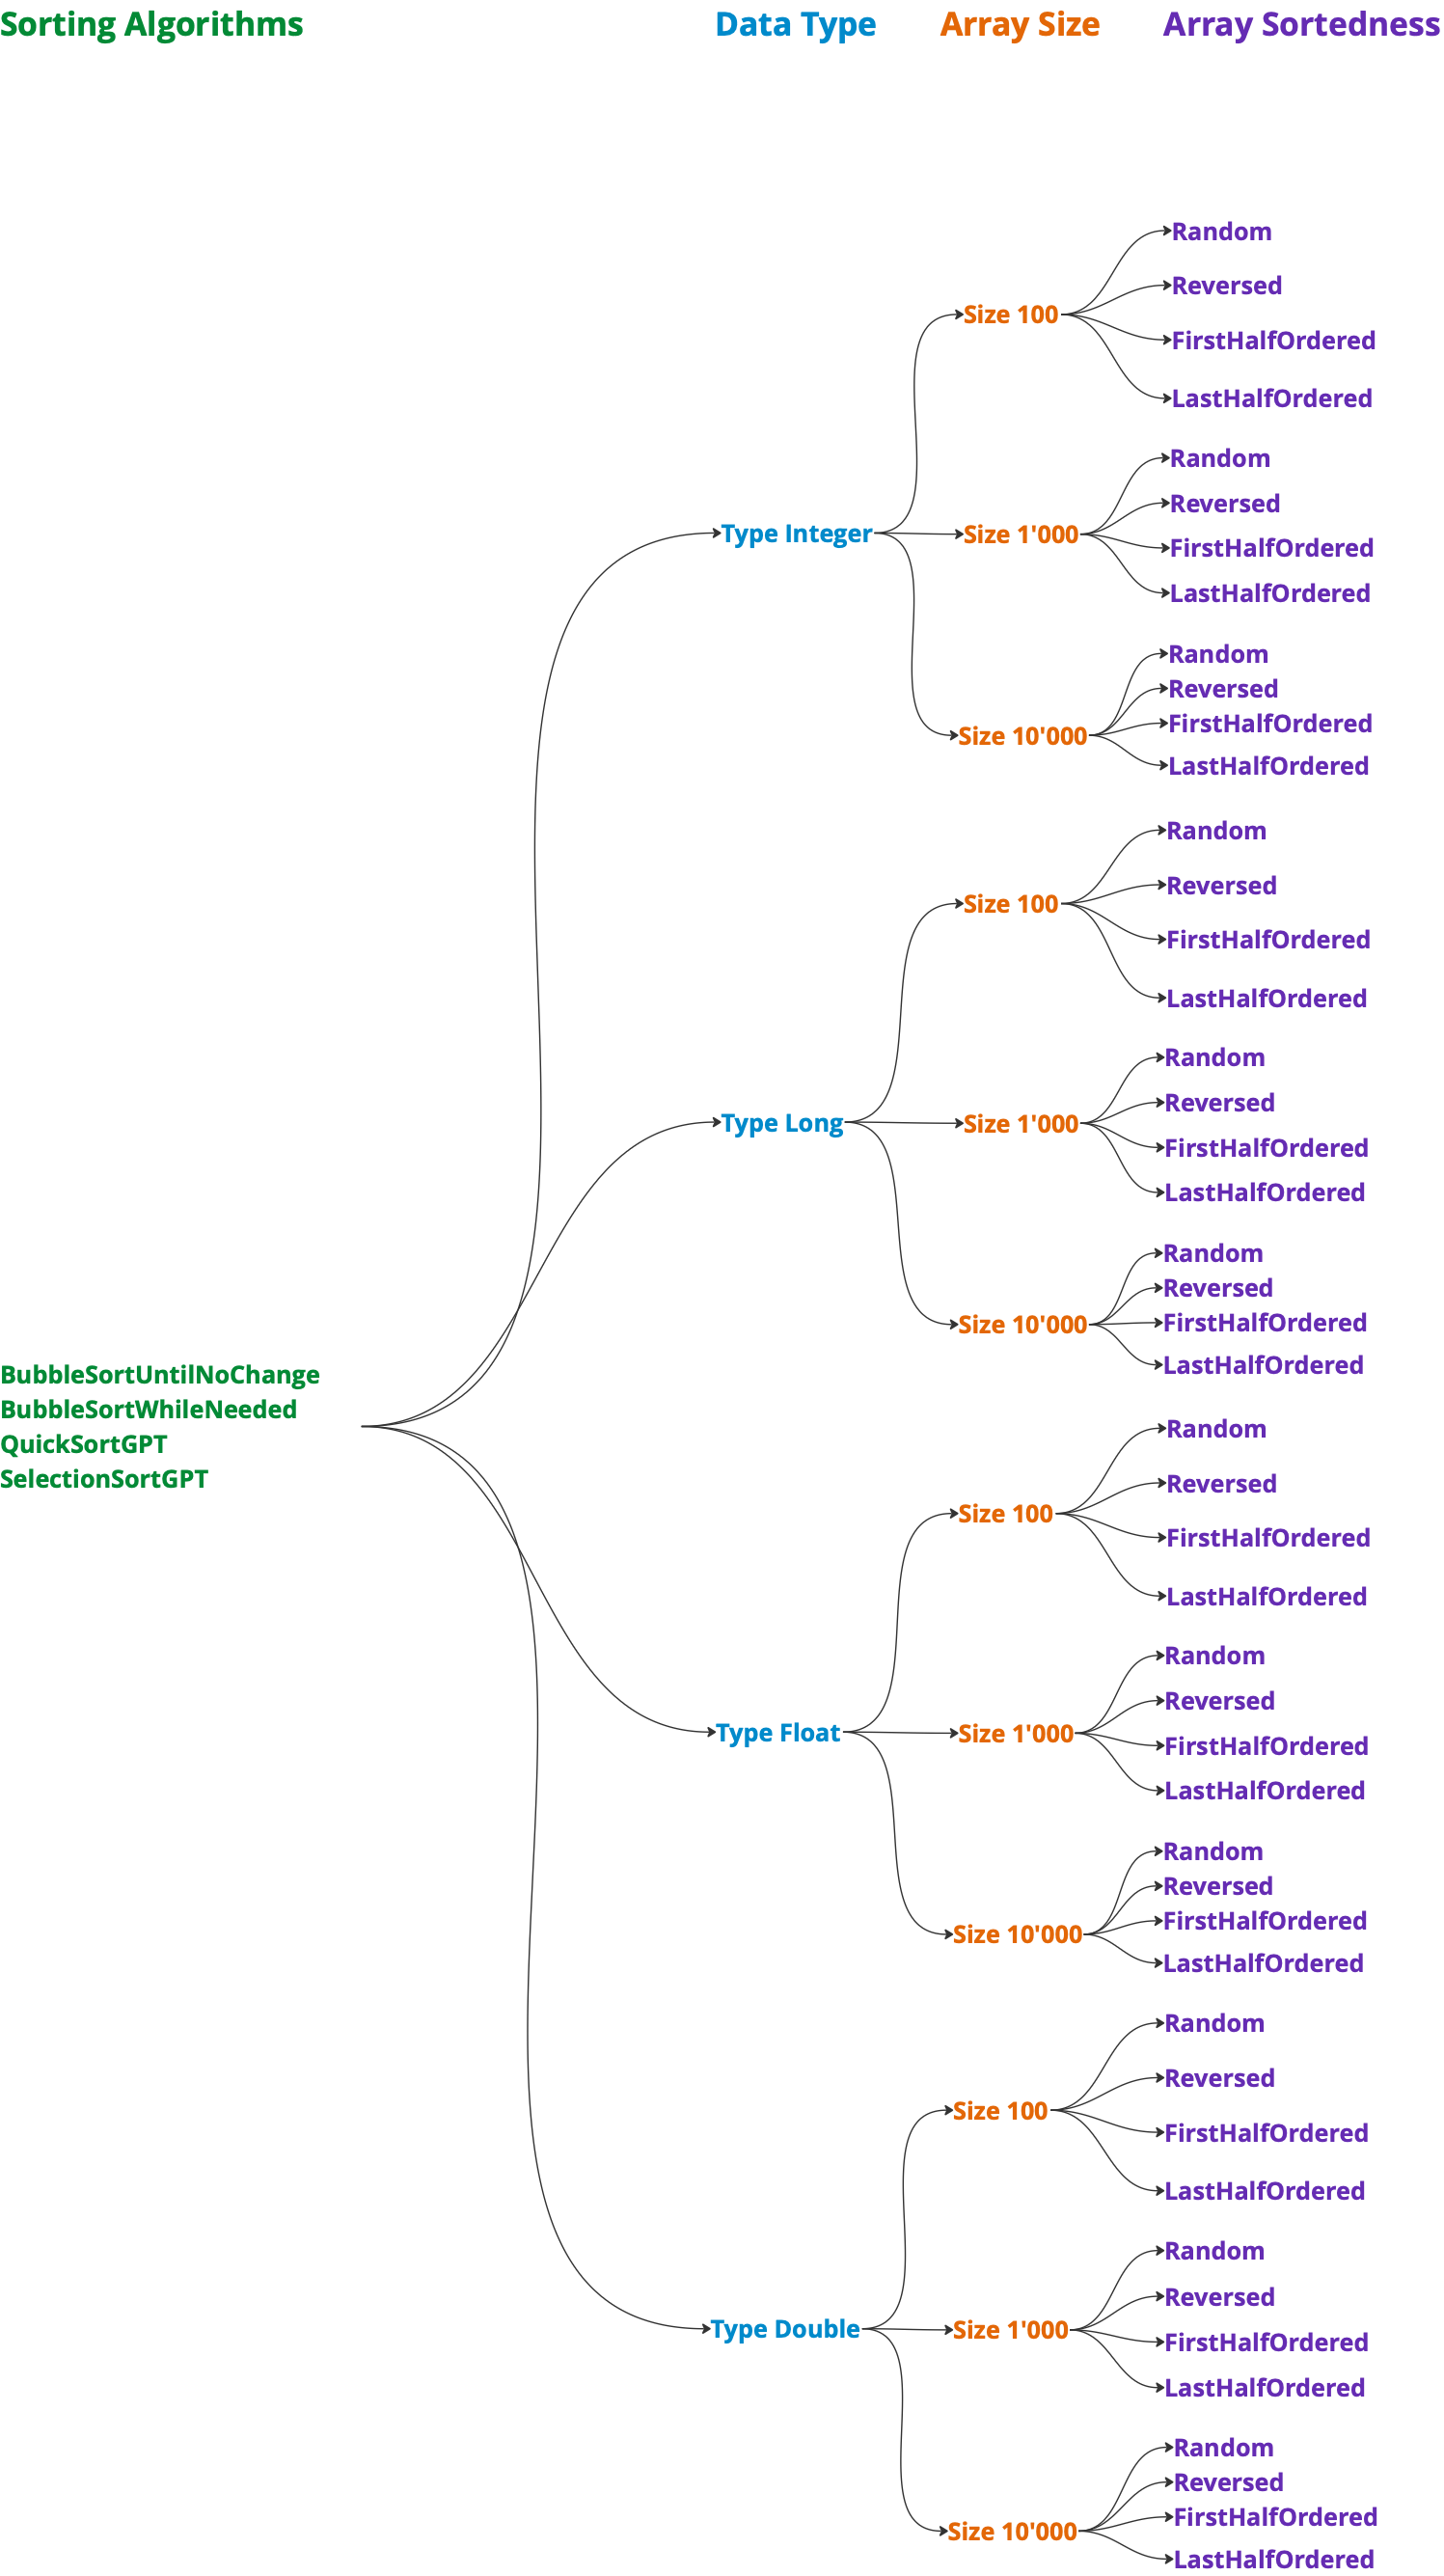
\includegraphics[width=0.8\textwidth]{./fig/factors.png}
            \caption{Factors in the experiment}
            \label{fig:factors}
        \end{figure}

    \end{itemize}

    \subsection{Apparatus and Materials}

    The experiment was conducted on a MacBook Air with an M1 chip, 8GB of RAM, running macOS Sequoia 15.1. The programming language used was OpenJDK 21.0.4, with VSCode version 1.92.1 as the integrated development environment (IDE). To ensure consistency and minimize interference, no other user processes were running in the background during the experiment.

    \subsection{Procedure}

    This is a high-level overview of the steps taken to conduct the experiment in terms of what the code does. \\

    \begin{enumerate}
        \item \textbf{Initialize Sorting Algorithms}:
        \begin{itemize}
            \item Define an array of sorting algorithms to test, each implementing a \texttt{sort} method (e.g., \texttt{BubbleSortUntilNoChange}, \texttt{BubbleSortWhileNeeded}, \texttt{QuickSortGPT}, \texttt{SelectionSortGPT}).
        \end{itemize}
    
        \item \textbf{Define Datasets}:
        \begin{itemize}
            \item Create datasets of varying sizes (100, 1,000, and 10,000) and data types (Integer, Long, Float, and Double).
            \item For each data type, initialize arrays for the specified sizes.
        \end{itemize}
    
        \item \textbf{Generate Dataset Configurations}:
        \begin{itemize}
            \item For each dataset, generate four initial configurations of data:
            \begin{itemize}
                \item \textbf{Random}: Populate the array with randomly generated values.
                \item \textbf{Reversed}: Populate the array with values in descending order.
                \item \textbf{First-half-sorted}: Sort the first half of the array, with the remaining elements randomized.
                \item \textbf{Last-half-sorted}: Sort the last half of the array, with the initial elements randomized.
            \end{itemize}
        \end{itemize}
    
        \item \textbf{Measure Execution Time}:
        \begin{itemize}
            \item For each sorting algorithm, dataset size, data type, and sortedness level, perform 100 timed sorting operations:
            \begin{itemize}
                \item Use \texttt{System.nanoTime()} to measure the execution time for each sort.
                \item Record the time taken in nanoseconds for each sort in a CSV file.
            \end{itemize}
        \end{itemize}
    
        \item \textbf{Store Results}:
        \begin{itemize}
            \item Record the algorithm name, data type, data size, sortedness level, and time taken for each run in the CSV file to allow for subsequent analysis.
        \end{itemize}
    
        \item \textbf{Analyze Data}:
        \begin{itemize}
            \item Process the CSV file using python3.12.4 in a Jupyter Notebook to create graphs and tables, analyzing the relationship between independent variables (sorting algorithm, data size, data type, and sortedness level) and the dependent variable (execution time).
        \end{itemize}
    \end{enumerate}


\section{Results}

    \subsection{Visual Overview}


    \begin{figure}[htbp]
        \centering
        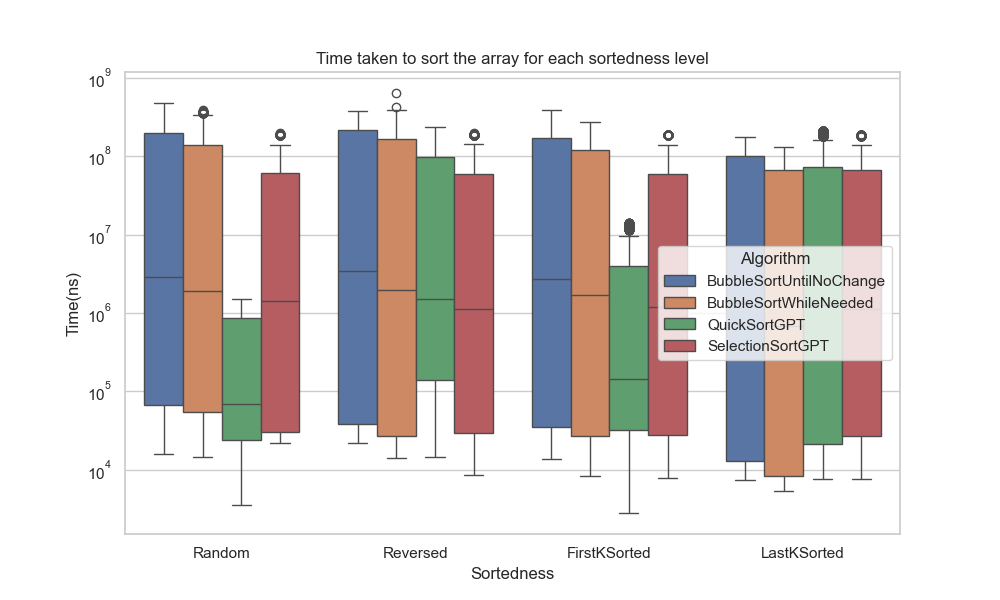
\includegraphics[width=0.8\textwidth]{./fig/hip1.png}
        \caption{Sortedness of input vs time in logarithmic scale}
        \label{fig:hip1}
    \end{figure}

    In Figure \ref{fig:hip1}, we show the relationship between the level of sortedness of the input data and the running time of the sorting algorithm. The x-axis represents the level of sortedness, while the y-axis (in logarithmic scale)represents the time in nanoseconds. The graph shows that the running time increases as the level of sortedness decreases. The relationship is also evident with the y-axis in linear scale, as shown in Figure \ref{fig:hip1_linear}.\\
    \hfill

    \begin{figure}[htbp]
        \centering
        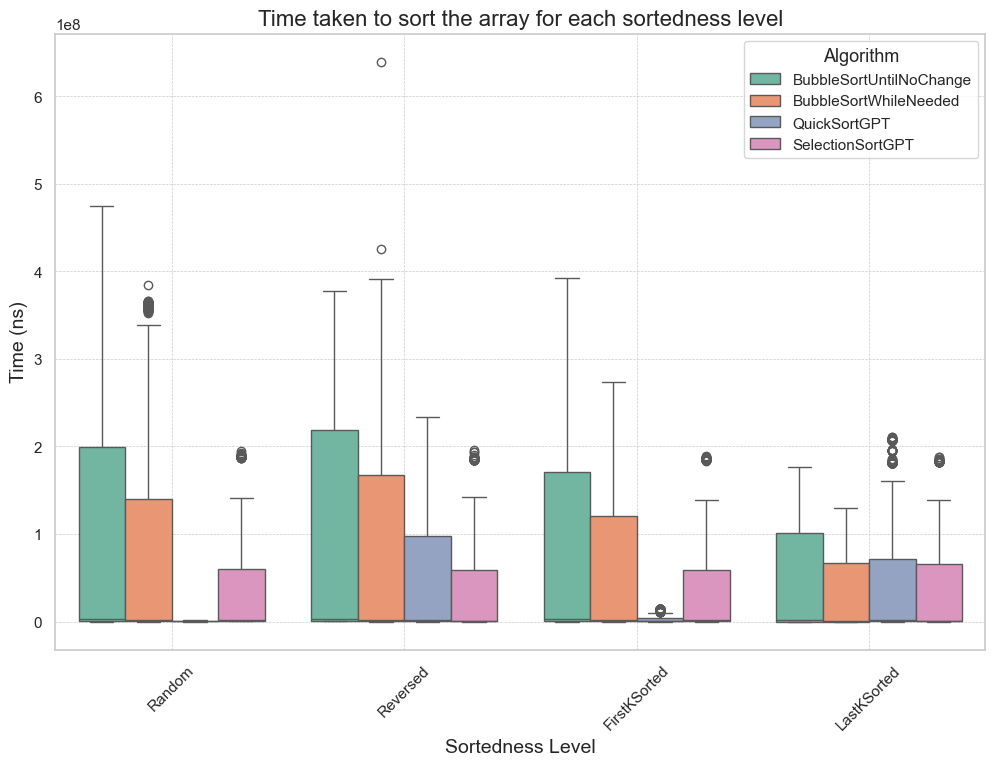
\includegraphics[width=0.8\textwidth]{./fig/hip1-nonLog.png}
        \caption{Sortedness of input vs time in linear scale}
        \label{fig:hip1_linear}
    \end{figure}

    In Figure \ref{fig:hip2}, we show the relationship between the size of the dataset and the running time of the sorting algorithm. The x-axis represents the size of the dataset, while the y-axis (in logarithmic scale) represents the time in nanoseconds. The graph shows that the running time increases as the size of the dataset increases. The relationship is more evident in the logarithmic scale.\\
\hfill



\begin{figure}[htbp]
    \centering
    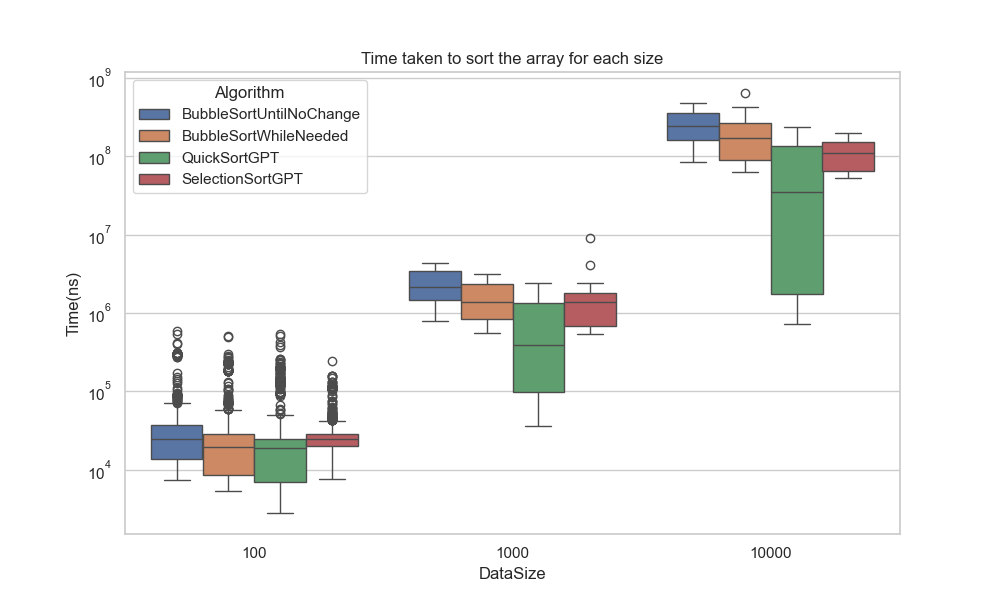
\includegraphics[width=0.8\textwidth]{./fig/hip2.png}
    \caption{Size of dataset vs time in logarithmic scale}
    \label{fig:hip2}
\end{figure}


    In Figure \ref{fig:hip3}, we show the relationship between the data type of the elements in the dataset and the running time of the sorting algorithm. The x-axis represents the data type, while the y-axis (in logarithmic scale) represents the time in nanoseconds. The graph shows that the running time varies across different data types, with Double (8B) having the highest running time. The relationship is more evident in the logarithmic scale.\\
\hfill
        \begin{figure}[htbp]
            \centering
            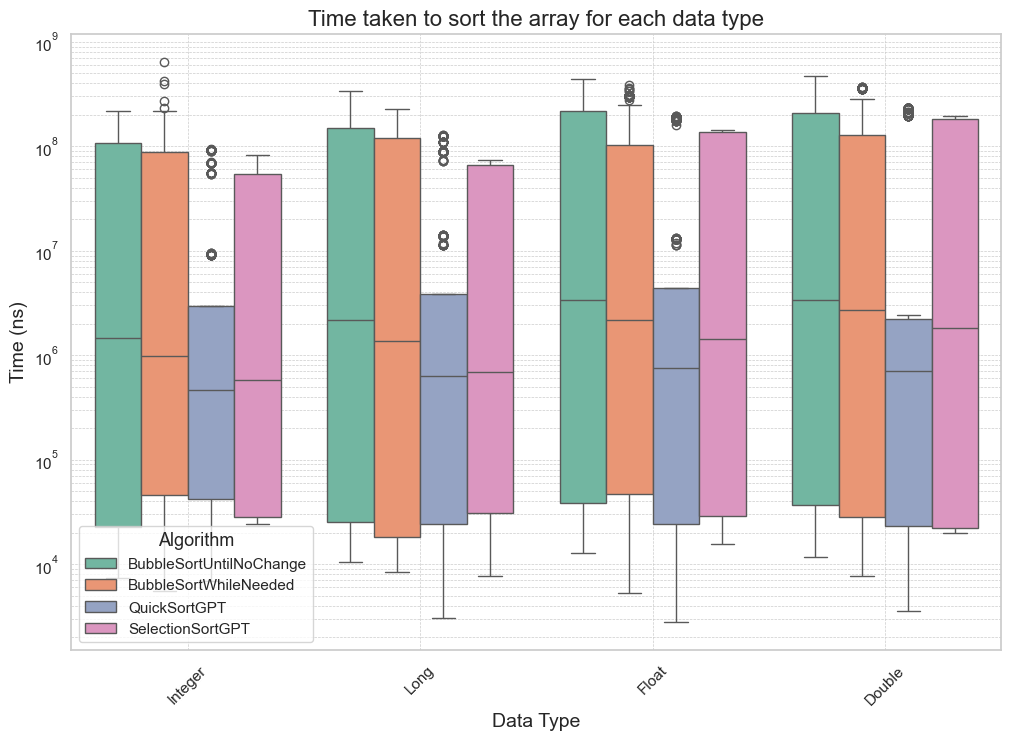
\includegraphics[width=0.8\textwidth]{./fig/hip3.png}
            \caption{Data type vs time in logarithmic scale}
            \label{fig:hip3}
        \end{figure}


    \subsection{Descriptive Statistics}
    Table \ref{descr_table} provides a summary of the running times for each sorting algorithm, data type, and sortedness level. The table includes the minimum, 1st quartile, median, 3rd quartile, and maximum values for the running times in nanoseconds. The data is grouped by Algorithm.\\
    \begin{center}
        \footnotesize
        \begin{longtable}{|l|l|l|r|r|r|r|r|}
            \hline
            \textbf{Algorithm} & \textbf{Sort} & \textbf{Type} & \textbf{min} & \textbf{1st Quartile} & \textbf{Median} & \textbf{3rd Quartile} & \textbf{max} \\
            \hline
            \endfirsthead
            \hline
            \textbf{Algorithm} & \textbf{Sort} & \textbf{Type} & \textbf{min} & \textbf{1st Quartile} & \textbf{Median} & \textbf{3rd Quartile} & \textbf{max} \\
            \hline
            \endhead
            \hline
            \endfoot
            \multirow{16}{*}{BSUNC} & FirstKSorted & Double & 34791.0 & 34875.0 & 3312062.0 & 343318844.0 & 351527666.0 \\
            & FirstKSorted & Float & 30750.0 & 31072.75 & 3155375.0 & 350424322.75 & 392856209.0 \\
            & FirstKSorted & Integer & 13583.0 & 14729.25 & 1343187.5 & 148487458.0 & 151545833.0 \\
            & FirstKSorted & Long & 20541.0 & 20989.75 & 2004687.5 & 234806093.75 & 335577375.0 \\
            & LastKSorted & Double & 11666.0 & 11750.0 & 1480958.0 & 160909833.25 & 165408292.0 \\
            & LastKSorted & Float & 12708.0 & 12958.0 & 1457250.0 & 167002396.0 & 176130916.0 \\
            & LastKSorted & Integer & 7333.0 & 7875.0 & 867541.5 & 91748813.0 & 97350042.0 \\
            & LastKSorted & Long & 10458.0 & 11062.25 & 1136354.5 & 122797698.0 & 125335375.0 \\
            & Random & Double & 32916.0 & 33042.0 & 3682646.0 & 424603208.0 & 474684667.0 \\
            & Random & Float & 30791.0 & 87791.75 & 3400917.0 & 422298510.25 & 439274584.0 \\
            & Random & Integer & 15666.0 & 133125.0 & 1492396.0 & 160357624.75 & 173614375.0 \\
            & Random & Long & 20583.0 & 66531.5 & 2178979.0 & 276661135.75 & 310634458.0 \\
            & Reversed & Double & 37000.0 & 37614.75 & 3387854.5 & 369365749.5 & 377215667.0 \\
            & Reversed & Float & 35334.0 & 38375.0 & 3646688.0 & 368913708.25 & 375371000.0 \\
            & Reversed & Integer & 21750.0 & 22584.0 & 1950646.0 & 205561052.25 & 215514250.0 \\
            & Reversed & Long & 23916.0 & 25333.0 & 2318750.0 & 257731780.75 & 262898583.0 \\
            \hline
            \multirow{16}{*}{BSWN} & FirstKSorted & Double & 26542.0 & 27770.5 & 2494000.0 & 269238020.75 & 273290750.0 \\
            & FirstKSorted & Float & 19291.0 & 19417.0 & 1994313.0 & 220615062.5 & 226031458.0 \\
            & FirstKSorted & Integer & 8208.0 & 8322.75 & 857646.0 & 94190728.75 & 109389625.0 \\
            & FirstKSorted & Long & 13375.0 & 14062.25 & 1201000.5 & 164325427.25 & 182960625.0 \\
            & LastKSorted & Double & 7750.0 & 8084.0 & 690875.0 & 79905770.75 & 82992583.0 \\
            & LastKSorted & Float & 5333.0 & 5417.0 & 573625.0 & 64216843.75 & 69149458.0 \\
            & LastKSorted & Integer & 5500.0 & 5625.0 & 590083.5 & 66779885.5 & 129658834.0 \\
            & LastKSorted & Long & 8334.0 & 8708.75 & 739145.5 & 81190062.25 & 111125875.0 \\
            & Random & Double & 28375.0 & 28583.0 & 3001229.5 & 359720093.5 & 366413042.0 \\
            & Random & Float & 46625.0 & 50239.5 & 2202333.0 & 300086094.0 & 384812458.0 \\
            & Random & Integer & 45042.0 & 47468.75 & 1002146.0 & 107917281.5 & 122899292.0 \\
            & Random & Long & 14458.0 & 59781.0 & 1402188.0 & 194750969.0 & 226067959.0 \\
            & Reversed & Double & 27083.0 & 27250.0 & 2690937.5 & 280814093.5 & 285547250.0 \\
            & Reversed & Float & 21625.0 & 24500.0 & 2434833.5 & 241278593.75 & 277258500.0 \\
            & Reversed & Integer & 13958.0 & 54562.0 & 1216875.0 & 153523864.75 & 639605292.0 \\
            & Reversed & Long & 17833.0 & 18042.0 & 1503917.0 & 167367146.25 & 171405667.0 \\
            \hline
            \multirow{16}{*}{QSGPT} & FirstKSorted & Double & 3791.0 & 3834.0 & 147187.5 & 1903906.0 & 2212208.0 \\
            & FirstKSorted & Float & 2792.0 & 3042.0 & 139333.0 & 12834749.75 & 13212750.0 \\
            & FirstKSorted & Integer & 32333.0 & 48875.0 & 102208.5 & 9286667.25 & 9579167.0 \\
            & FirstKSorted & Long & 3083.0 & 3167.0 & 151167.0 & 13716134.75 & 14160542.0 \\
            & LastKSorted & Double & 21166.0 & 22000.0 & 1955250.5 & 207200749.75 & 211028916.0 \\
            & LastKSorted & Float & 17042.0 & 17209.0 & 1840125.0 & 181340145.5 & 185499167.0 \\
            & LastKSorted & Integer & 7500.0 & 93739.5 & 561541.5 & 68887509.75 & 71272667.0 \\
            & LastKSorted & Long & 10250.0 & 10292.0 & 739646.0 & 88561885.0 & 90974583.0 \\
            & Random & Double & 3583.0 & 3875.0 & 81479.5 & 1250177.25 & 1462875.0 \\
            & Random & Float & 23792.0 & 24280.75 & 69708.0 & 1170760.25 & 1494041.0 \\
            & Random & Integer & 6875.0 & 7655.75 & 37562.5 & 740969.0 & 839833.0 \\
            & Random & Long & 23291.0 & 24041.75 & 53792.0 & 887865.0 & 1327291.0 \\
            & Reversed & Double & 23375.0 & 23500.0 & 2221333.5 & 229394791.5 & 234112417.0 \\
            & Reversed & Float & 18250.0 & 136677.75 & 1893042.0 & 188588510.75 & 195573416.0 \\
            & Reversed & Integer & 41584.0 & 195208.0 & 765833.5 & 91154051.75 & 93264417.0 \\
            & Reversed & Long & 14459.0 & 141229.0 & 1109583.0 & 125214010.25 & 127176375.0 \\
            \hline
            \multirow{16}{*}{SSGPT} & FirstKSorted & Double & 21875.0 & 22583.0 & 1841437.5 & 184498437.5 & 188602875.0 \\
            & FirstKSorted & Float & 17291.0 & 29989.5 & 1423271.0 & 136545218.75 & 138658833.0 \\
            & FirstKSorted & Integer & 27541.0 & 28334.0 & 580250.0 & 54831750.0 & 56596041.0 \\
            & FirstKSorted & Long & 7833.0 & 7989.75 & 688000.5 & 65361333.5 & 66988292.0 \\
            & LastKSorted & Double & 20208.0 & 21030.75 & 1805854.5 & 182897791.0 & 188457666.0 \\
            & LastKSorted & Float & 15583.0 & 15875.0 & 1388062.5 & 136043916.75 & 138951667.0 \\
            & LastKSorted & Integer & 26667.0 & 28198.5 & 582562.0 & 55050457.75 & 82011875.0 \\
            & LastKSorted & Long & 7666.0 & 8250.0 & 688687.5 & 65729291.25 & 68346333.0 \\
            & Random & Double & 21791.0 & 21917.0 & 1861292.0 & 187903781.25 & 195235792.0 \\
            & Random & Float & 28375.0 & 28697.75 & 1420229.0 & 136688541.75 & 140796417.0 \\
            & Random & Integer & 26583.0 & 27239.75 & 582875.0 & 55168385.75 & 58463000.0 \\
            & Random & Long & 30166.0 & 109656.5 & 690541.5 & 65995281.25 & 68053875.0 \\
            & Reversed & Double & 19708.0 & 19792.0 & 1827187.5 & 184536437.75 & 195752416.0 \\
            & Reversed & Float & 26375.0 & 43083.0 & 1391958.5 & 137661250.25 & 142159416.0 \\
            & Reversed & Integer & 24459.0 & 25375.0 & 540395.5 & 53358979.25 & 55007000.0 \\
            & Reversed & Long & 8500.0 & 30989.75 & 735229.0 & 72350291.0 & 74371750.0 \\
            \hline
                    \caption{Descriptive statistics summary}
        \label{descr_table}
        \end{longtable}
    \end{center}



\section{Discussion}

    \subsection{Compare Hypotheses with Results}

    We decided to use the median as our statistic of interest when discussing the resuls because it is less affectd by extreme values which, in our case, may due to system-dependent causes such as job scheduling and it reflects the typical behaviour of a phenomenon, in our case the algorithm.

    When observing the plots we can see that, overall, the median trends seem to be consistent across the various independent variables explored: both BubbleSortUntilNoChange and BubbleSortWhileNeeded appear to be the slowest, followed by SelectionSortGPT and QuickSortGPT usually peforms better than the others. 

    Now we discuss the median values with respect to each hypothesis:

    \begin{enumerate}
        \item Hypothesis 1: \textit{ The level of sortedness of the input data impacts the running time of the sorting algorithm}. As shown in Figure \ref{fig:hip1} and \ref{fig:hip1_linear} we can see that QuickSort performs better with Random and FirstKSorted sortings, while with Reversed sorting we see SelectionSortGPT peform slightly faster. The rest of the algorithms seem to not be as affecte the level of sortedness of the input data, suggesting that the only algorithm out of the four we analyzed that is sensitive to the level of sortedness is QuickSortGPT.

        \item Hypothesis 2: \textit{The size of the dataset impacts the running time of the sorting algorithm}. As shown in Figure \ref{fig:hip2} we observe that overall, all the algorithms perform better with smaller arrays, which makes sense because there is less data to process. What seems to be the most relevant finding here is that QuickSortGPT is particularly faster compared to the others with large datasets.

        \item Hypothesis 3: \textit{The data type of the elements in the dataset impacts the running time of the sorting algorithm}. When looking at \ref{fig:hip3} we can see how the performance of all of the four algorithms remains consistent with all the analyzed data types. Integer and Long data dypes appear to have a very slight better performance but these findings suggest that the data types that were analyzed in this experiment don't have a relevant impact on the dependent variable.
    \end{enumerate}


    \subsection{Limitations and Threats to Validity}

    Limitations of this study could be the folowing:
    \begin{itemize}
        \item Analysis: we only considered the median and we did not perform any inferential statistics to determine the actual relevance of our findings
        \item Execution: we exclusivly ran the experiment on one specific system, not exploring the impact of using different hardware and software
    \end{itemize}

    Threats to validity are mainly related to the experiment being performed on a single harware and software combination.



    \subsection{Conclusions}

    This study explored the effects of input sortedness, dataset size, and data type on the performance of four provided sorting algorithms: BubbleSortUntilNoChange, BubbleSortWhileNeeded, SelectionSortGPT, and QuickSortGPT. Using the median of running times to account for system variability, we found that QuickSortGPT consistently outperformed the other algorithms, particularly on larger datasets. SelectionSortGPT was moderately efficient, while the BubbleSort variants were consistently slower.

    In particular: QuickSortGPT was sensitive to input sortedness, performing best on random and partially sorted data, while SelectionSortGPT slightly outperformed QuickSortGPT on reversed data. All algorithms performed better with smaller datasets, with QuickSortGPT showing the greatest advantage as size increased. Data type had minimal impact on performance.


\section{Appendix}

    \subsection{Reproduction Package}
    All of the code used to conduct the experiment, as well as the Jupyter Notebook used for data analysis and the Latex files for the report, can be found at the following GitHub repository: \url{https://github.com/costanza1234/USI-Exp-Eval-24}.

\end{document}